\section{Twin Calibration and first results with the twin}
\label{section:twin}

\paragraph{Method.} For every patient, the twin is calibrated on the first 5 minutes of the recording, without using any labels: we take the patient's median beat and fit the 15 wave parameters of the McSharry model \cite{mcsharry2003dynamical}, together with a gain and an offset, by nonlinear least squares. On synthetic beats with known parameters, this procedure recovered the true beat to within the added noise in all nine tests, at three different heart rates. For each later beat, the deviation score $d_k$ compares the beat with the twin's beat, relative to the patient's own beat-to-beat variation, so a typical beat has $d_k \approx 1$. As a control we compute the same score against the patient's raw median beat, i.e.\ without the physiological model.

\paragraph{Calibration.} Across the 43 patients, the calibrated twin reproduces the patient's median beat with a median error of 0.032~mV, against 0.181~mV for the uncalibrated population twin (Figure~\ref{fig:twin}, left).

\begin{figure}[H]
\centering
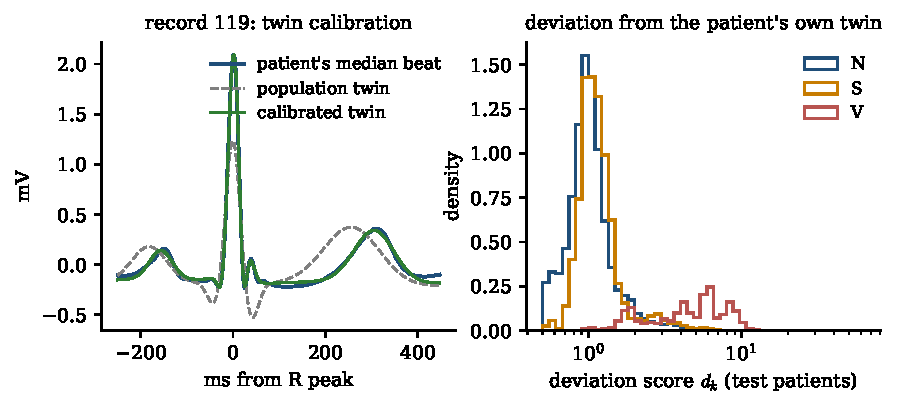
\includegraphics[width=0.88\textwidth]{Fig/s4_twin.pdf}
\caption{Left: twin calibration for one patient. Right: deviation scores of all test beats after calibration; ventricular beats stand out, supraventricular beats do not.}
\label{fig:twin}
\end{figure}

\paragraph{Deviation score.} On the test patients, normal beats have a median deviation of 1.07 and ventricular beats 6.09 (Figure~\ref{fig:twin}, right). The score alone separates ventricular from normal beats with an AUROC of 0.98, but supraventricular beats only weakly (0.60), because their shape is almost normal. The model-free control scores the same for ventricular beats (0.98) and slightly lower for supraventricular ones (0.57).

\paragraph{Does the twin help the classifier?} We add the deviation score as an extra feature to the baseline classifier and compare it with the same classifier without it. For a fair comparison, both are trained only on beats after the first 5 minutes, which is why the baseline differs slightly from Table~\ref{tab:detection}. Since each patient is one independent unit, we give 95\% intervals from a bootstrap over the 21 test patients (Table~\ref{tab:ablation}).

\begin{table}[H]
\caption{Effect of the deviation score on the baseline classifier (test patients). Differences are relative to the classifier without the score, with 95\% bootstrap intervals over patients.}
\label{tab:ablation}
\centering
\small
\setstretch{1.1}
\begin{tabular}{@{}lccc@{}}
\toprule
 & \textbf{Without score} & \textbf{+ twin score} & \textbf{+ control score} \\
\midrule
Macro-F1 & 0.538 & 0.561 & 0.537 \\
\quad difference & -- & $+0.036$ [$-0.021$, $0.110$] & $+0.008$ [$-0.031$, $0.056$] \\
F1, ventricular (V) & 0.879 & 0.956 & 0.943 \\
\quad difference & -- & $+0.085$ [$0.022$, $0.205$] & $+0.073$ [$0.017$, $0.191$] \\
F1, supraventricular (S) & 0.309 & 0.224 & 0.216 \\
\quad difference & -- & $-0.060$ [$-0.177$, $0.097$] & $-0.070$ [$-0.199$, $0.101$] \\
\bottomrule
\end{tabular}
\end{table}

\paragraph{Discussion.} Personalisation clearly helps where shape matters. With the twin's score, ventricular beats are detected far more precisely (F1 0.88 $\rightarrow$ 0.96), and this gain is consistent across patients. The overall macro-F1 also rises, but with only 21 test patients the interval still includes zero, so we cannot yet claim an overall improvement. Supraventricular beats are not helped, which matches the data: they differ from normal beats in timing, not in shape. On detection alone, the physiological twin performs about as well as the model-free control. Its added value is that its parameters have a meaning (for example the width of the QRS complex) and that it can simulate the patient, which the next stages will use for the clinical report. Next steps are to combine the score with the CNN, add timing to the twin, and test on a wearable dataset.
